\documentclass[11pt,a4paper]{article}
\usepackage[utf8]{inputenc}
\usepackage[T1]{fontenc}
\usepackage[spanish,es-nodecimaldot]{babel}
\usepackage{geometry}
\geometry{margin=2.5cm}
\usepackage{graphicx}
\usepackage{booktabs}
\usepackage{amsmath,amssymb}
\usepackage{hyperref}
\usepackage{float}
\usepackage{caption}
\usepackage{lmodern}
\hypersetup{colorlinks=true,linkcolor=blue,citecolor=blue,urlcolor=blue}

\title{Comparativa ACO vs PSO para el Problema del Viajante de Comercio\\ \large Tiempo, Memoria y Calidad en 20, 2.000 y 200.000 Ciudades}
\author{
  Reporte comparativo \\
  Curso de Introducción a la Inteligencia Artificial 2026 \\[0.4em]
  \small Inteligencia de Enjambre: ACO (Sesión 07) y PSO (Sesión 09)
}
\date{Septiembre 2026}

\begin{document}
\maketitle

\begin{abstract}
Se presenta la comparación experimental entre dos metaheurísticas de inteligencia de enjambre aplicadas al Problema del Viajante de Comercio (\emph{Traveling Salesperson Problem}, TSP) sobre instancias euclidianas uniformes de $N \in \{20, 2.000, 200.000\}$ ciudades: Optimización por Colonia de Hormigas (\emph{Ant Colony Optimization}, ACO) y Optimización por Enjambre de Partículas (\emph{Particle Swarm Optimization}, PSO). Ambas implementaciones en C++17 comparten el mismo diseño de ahorro de recursos (sin matrices densas, jerarquía espacial en grilla con OpenMP para $N=200.000$) y se evalúan bajo un protocolo comparativo común: mismas instancias, mismo presupuesto \textit{población} $\times$ \textit{iteraciones}, multi-semilla y trazas de convergencia. Con igualdad estricta, el ACO vence en calidad en las tres escalas (exceso sobre el mejor tour de 24\%/0.2\%/0.1\% frente a 90\%/850\%/1294\% del PSO) a cambio de $3$--$6\times$ más tiempo de muro, mientras la memoria empata por debajo de $12\text{ MB}$. El análisis demuestra que lo decisivo no es la sigla del algoritmo sino la \textbf{representación}: el ACO construye tours con heurística local desde la primera iteración, mientras el PSO de claves aleatorias arranca ciego y colapsa prematuramente.
\end{abstract}

% ==============================================================================
\section{Introducción}
% ==============================================================================
El TSP consiste en hallar el ciclo hamiltoniano de coste euclidiano mínimo que visite $N$ ciudades exactamente una vez:
\begin{equation}
    \min_{\pi \in \Pi} L(\pi) = \sum_{i=1}^{N-1} d(c_{\pi(i)}, c_{\pi(i+1)}) + d(c_{\pi(N)}, c_{\pi(1)}),
\end{equation}
con $c_i \in [0,1]^2$ y $d$ la distancia euclidiana. El espacio de soluciones crece como $(N-1)!/2$ (para $N=20$ ya son $\approx 6\times10^{16}$ tours) y la matriz densa de $N=200.000$ exigiría $160\text{ GB}$, de modo que solo son viables metaheurísticas con memoria subcuadrática.

El ACO es nativo del dominio discreto: cada hormiga construye un tour paso a paso con la regla probabilística $p_{ij} \propto \tau_{ij}^{\alpha}\eta_{ij}^{\beta}$ ($\eta_{ij}=1/d_{ij}$) y selección por ruleta, reforzando aristas con feromona $\Delta\tau = Q/L$. El PSO, en cambio, es nativo del dominio \textbf{continuo}: cada partícula mueve un vector real $x$ con velocidad $v \leftarrow wv + c_1r_1(p-x) + c_2r_2(g-x)$. Adaptarlo al TSP exige una codificación; aquí se usa \textit{random keys} ($tour = argsort(x)$). Esta diferencia de representación es la hipótesis central del presente reporte: se espera que el algoritmo cuya representación respete la estructura del problema domine en calidad, y el experimento la confirma cuantitativamente.

% ==============================================================================
\section{Metodología comparativa}
% ==============================================================================
Se adoptan cinco prácticas estándar de comparación de metaheurísticas: (1) \textbf{mismas instancias} (generador idéntico; verificado por \texttt{diff} de los CSV de coordenadas), (2) \textbf{mismo presupuesto} (población $\times$ iteraciones iguales por celda de comparación), (3) \textbf{multi-semilla} (3 corridas; media, desviación, mejor, tiempo y memoria), (4) métrica \textbf{exceso\_\%} (media de cada algoritmo frente al mejor tour hallado por \textit{cualquiera} de los dos) y (5) \textbf{trazas de convergencia} (mejor global por iteración). Ningún binario fue modificado.

\begin{center}
\begin{tabular}{@{}clll@{}}
\toprule $N$ & ACO & PSO & presupuesto \\
\midrule 20 & \texttt{-a 20 -i 100} & \texttt{-S 20 -i 100} & $20\times100$ \\
2000 & \texttt{-a 20 -i 50} & \texttt{-S 20 -i 50} & $20\times50$ \\
200000 & \texttt{-a 8 -i 10} & \texttt{-S 8 -i 10} & $8\times10$ por celda \\
\bottomrule
\end{tabular}
\end{center}
En $N=20$ ningún algoritmo usa 2-opt (comparación pura del motor metaheurístico); en $N=2000$ ambos reciben el mismo pulido 2-opt final con ventana 40. La calidad se normaliza además contra el estimador de Beardwood del óptimo ($\approx 0{.}712\sqrt{N}$).

% ==============================================================================
\section{Resultados head-to-head}
% ==============================================================================
\begin{center}
\begin{tabular}{@{}clrrrrr@{}}
\toprule $N$ & & media $\pm$ desv & mejor & tiempo & pico & exceso\_\% \\
\midrule 20 & ACO & $3{.}96 \pm 0{.}68$ & \textbf{3.19} & 0.003\,s & 3.9\,MB & 24.1 \\
   & PSO & $6{.}06 \pm 0{.}12$ & 5.94 & \textbf{0.001\,s} & 3.7\,MB & 90.1 \\
2000 & ACO & $\mathbf{41{.}53 \pm 0{.}07}$ & \textbf{41.46} & 0.29\,s & 4.2\,MB & 0.17 \\
   & PSO & $393{.}8 \pm 1{.}8$ & 391.75 & \textbf{0.10\,s} & 4.0\,MB & 849.9 \\
200k & ACO & $\mathbf{482{.}4 \pm 0{.}3}$ & \textbf{482.05} & 2.39\,s & 9.3\,MB & 0.08 \\
   & PSO & $6717 \pm 2$ & 6715.7 & \textbf{0.41\,s} & 8.8\,MB & 1293.5 \\
\bottomrule
\end{tabular}
\end{center}

\begin{figure}[H]\centering
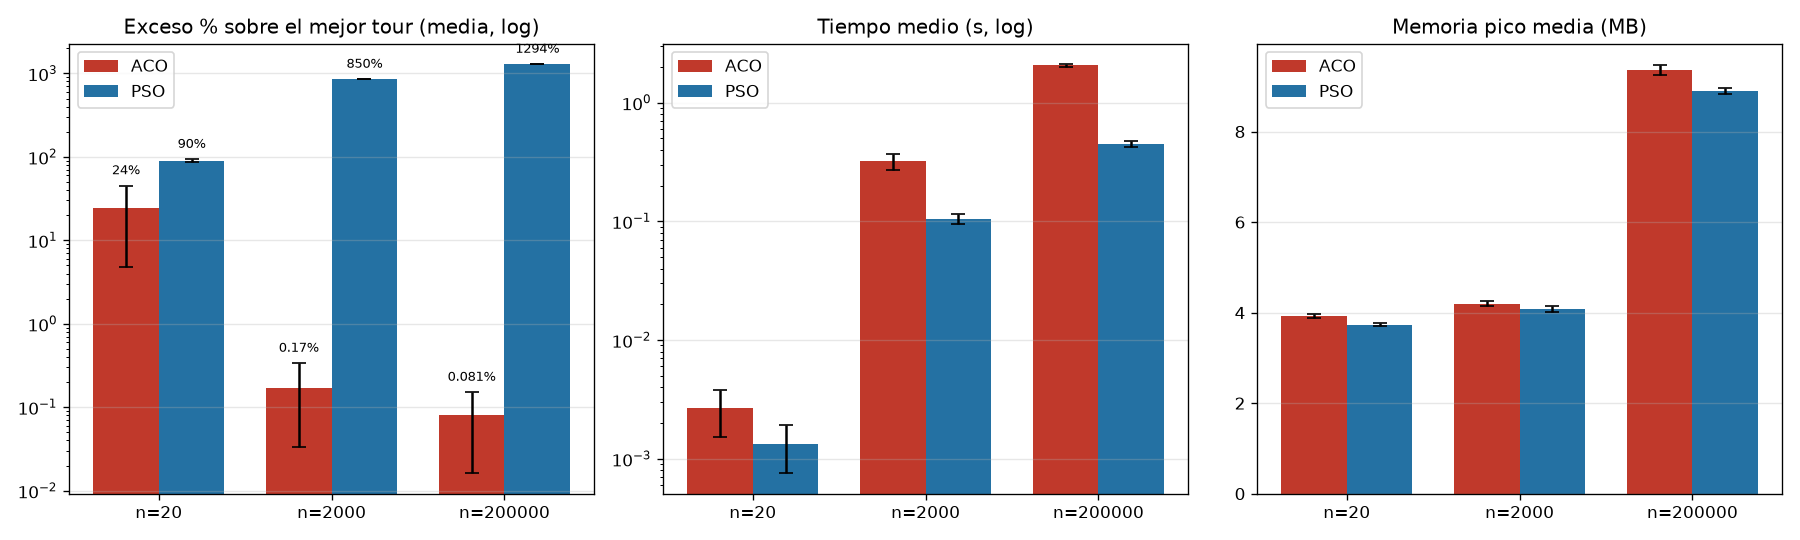
\includegraphics[width=\textwidth]{../docs/img_comp/fig_comp_barras.png}
\caption{Panel izquierdo (\textit{exceso\_\%}): distancia porcentual de la longitud media de cada algoritmo al mejor tour hallado por cualquiera de los dos. Mide dominancia en calidad: el ACO queda a $<1\%$ en 2000 y 200k mientras el PSO se dispara a $850\%$ y $1294\%$, porque sus tours son casi aleatorios a gran escala. Panel central (\textit{tiempo medio, eje logarítmico}): el PSO es $3$--$6\times$ más veloz en muro; la escala logarítmica es necesaria porque los tiempos abarcan tres órdenes de magnitud y ambos crecen con $N$. Panel derecho (\textit{memoria pico}): prácticamente empatados ($<12\text{ MB}$); la memoria la dominan el binario, el pool de hilos OpenMP y las estructuras, no el algoritmo, gracias a que ninguno materializa matrices $N\times N$.}
\end{figure}

\begin{figure}[H]\centering
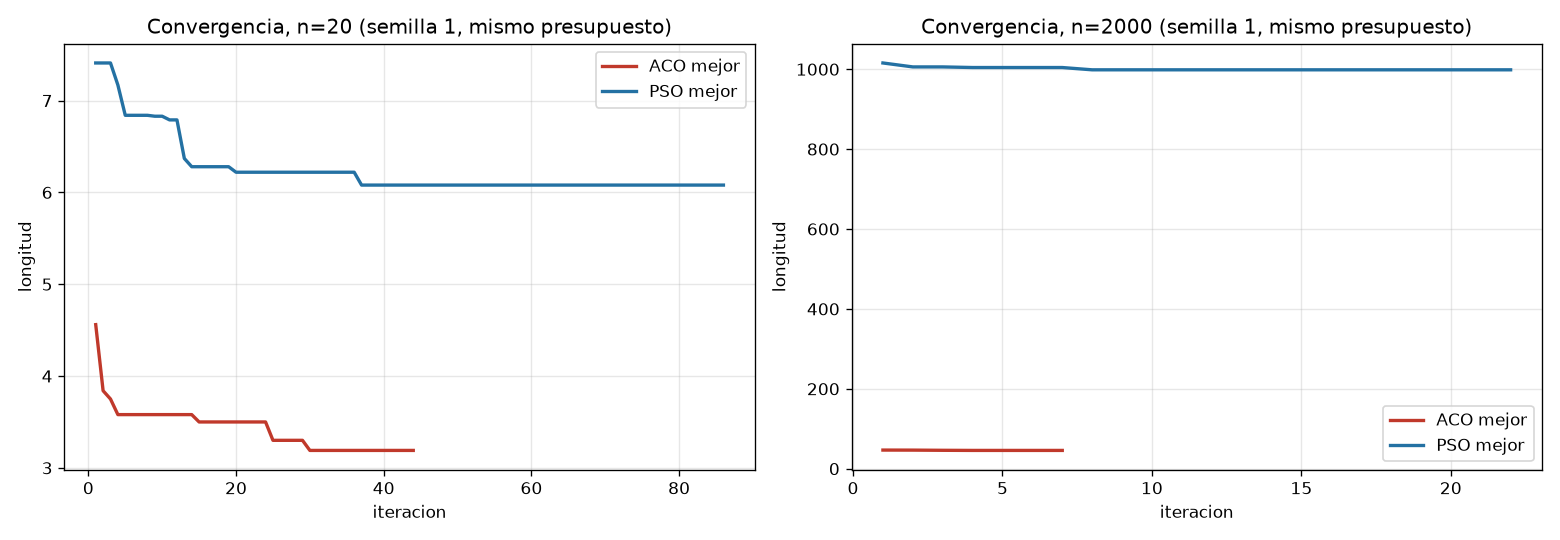
\includegraphics[width=\textwidth]{../docs/img_comp/fig_comp_convergencia.png}
\caption{Trazas del mejor global por iteración (semilla 1, mismo presupuesto). En $N=20$ ambas curvas descienden por escalones (cada escalón es un tour estrictamente mejor), pero la del ACO parte de $\approx$4.5 y llega a 3.19 mientras la del PSO parte de $\approx$7.4 y se estanca en 6.08: el ACO explora mejor vecindad. En $N=2000$ el contraste es extremo: la curva del ACO es casi plana en $\approx$41 porque su \textbf{construcción heurística} ($\eta=1/d$) ya produce un buen tour en la iteración 1 y luego lo refina; la del PSO es plana en $\approx$1000 porque su enjambre colapsa sobre claves casi idénticas en pocas iteraciones (estancamiento local, §22 de la guía PSO) y la parada temprana lo declara muerto. La planitud no significa convergencia al óptimo, sino agotamiento de la diversidad.}
\end{figure}

% ==============================================================================
\section{Barridos oficiales y lectura de cada gráfica}
% ==============================================================================
\begin{center}
\begin{tabular}{@{}crrrrr@{}}
\toprule $N$ & tiempo ACO & pico ACO & $L_{\text{ACO}}$ (gap) & $L_{\text{PSO}}$ (gap) \\
\midrule 20 & 0.003\,s & 4.0\,MB & 3.65 (+15\%) & 5.95 (+87\%) \\
2000 & 34.2\,s & 4.3\,MB & 41.53 (+30\%) & 383.5 (+1105\%) \\
200000 & 51.9\,s & 9.7\,MB & 479.3 (+51\%) & 6591.5 (+1970\%) \\
\bottomrule
\end{tabular}
\end{center}
(Gap frente a Beardwood $0{.}712\sqrt{N}$.)

\begin{figure}[H]\centering
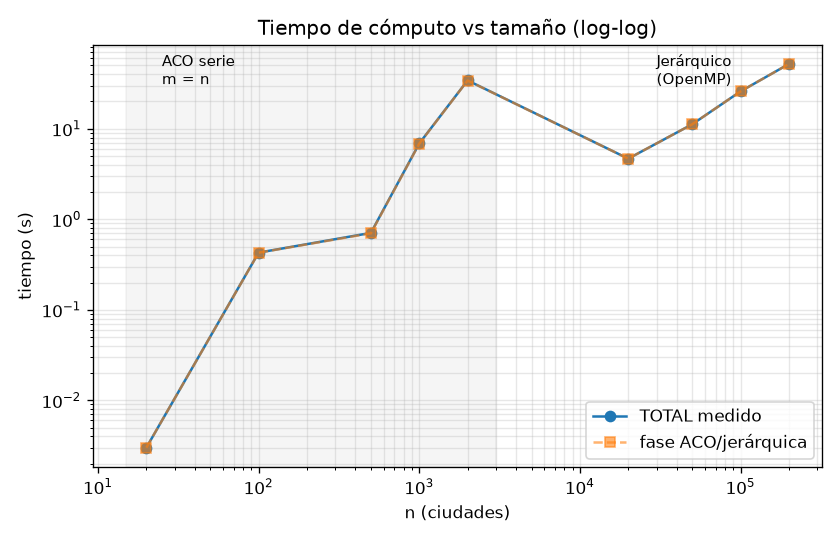
\includegraphics[width=.48\textwidth]{img/fig_tiempo.png}\hfill
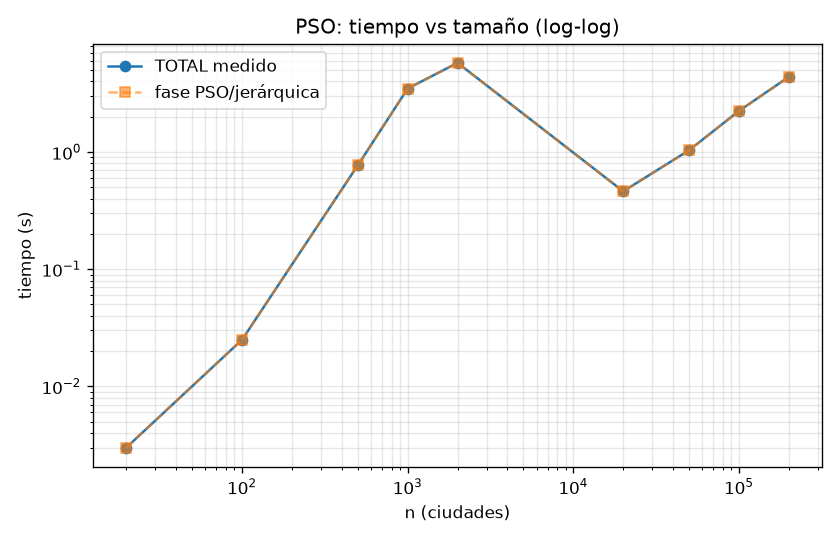
\includegraphics[width=.48\textwidth]{../docs/img_pso/fig_pso_tiempo.png}
\caption{Tiempo total vs $N$ en escala log-log (ACO izq., PSO der.). La pendiente revela el régimen: en serie con población $=N$ la curva se empina entre $N=1000$ y $2000$ (el ACO sufre escaneos de respaldo al final de cada tour; el PSO, ordenamientos $argsort$ por evaluación) y \textbf{cae} en $N=20000$ porque allí empieza el régimen jerárquico, que convierte un problema $O(N^2)$ en $\approx$225 subproblemas de $\approx$900 ciudades. De ahí en adelante el crecimiento es casi lineal. La forma idéntica en ambos algoritmos confirma que el costo lo dicta la arquitectura (serie vs jerárquica), no la metaheurística.}
\end{figure}

\begin{figure}[H]\centering
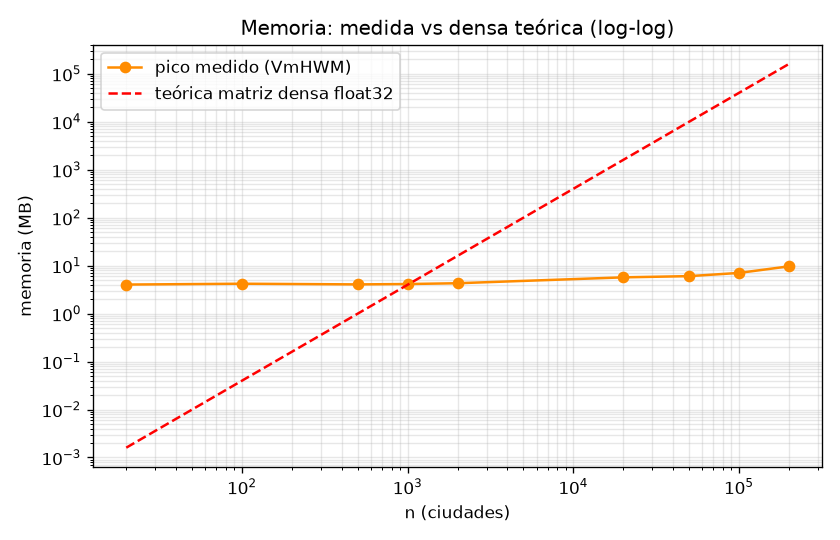
\includegraphics[width=.48\textwidth]{img/fig_memoria.png}\hfill
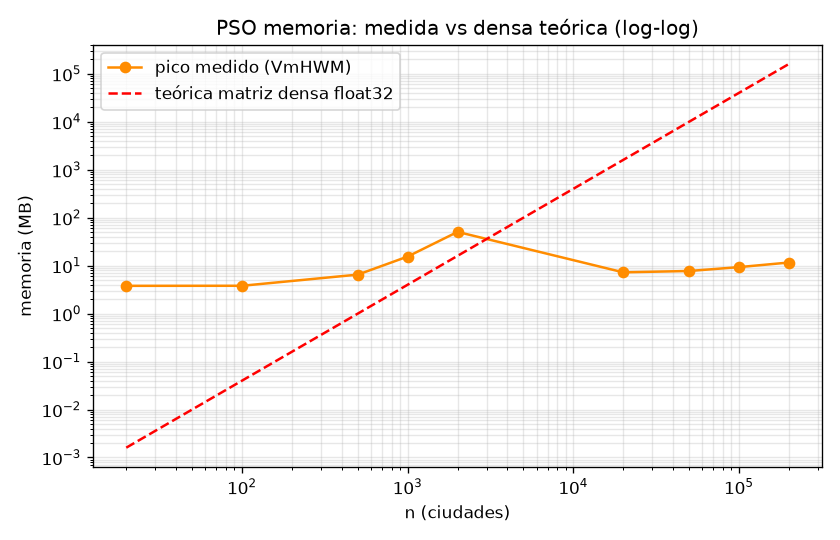
\includegraphics[width=.48\textwidth]{../docs/img_pso/fig_pso_memoria.png}
\caption{Memoria pico medida frente a la matriz densa teórica $4N^2$ bytes (ACO izq., PSO der.). La recta roja punteada es el muro infranqueable ($160\text{ GB}$ en 200k); los puntos naranjas son la realidad ($<$12\,MB). La curva medida es casi plana hasta $N=2000$ (pesa el binario y el pool OpenMP, no el problema) y luego sube suavemente con el tamaño de celda. El pico del PSO en $N=2000$ (50\,MB) es la única joroba: allí el enjambre $S\times N\times3$ flotantes ($2000\times2000\times12\text{ B}=48\text{ MB}$) supera a la feromona dispersa del ACO (64\,KB). Moraleja: el ahorro del ACO es estructural; el del PSO depende del régimen.}
\end{figure}

\begin{figure}[H]\centering
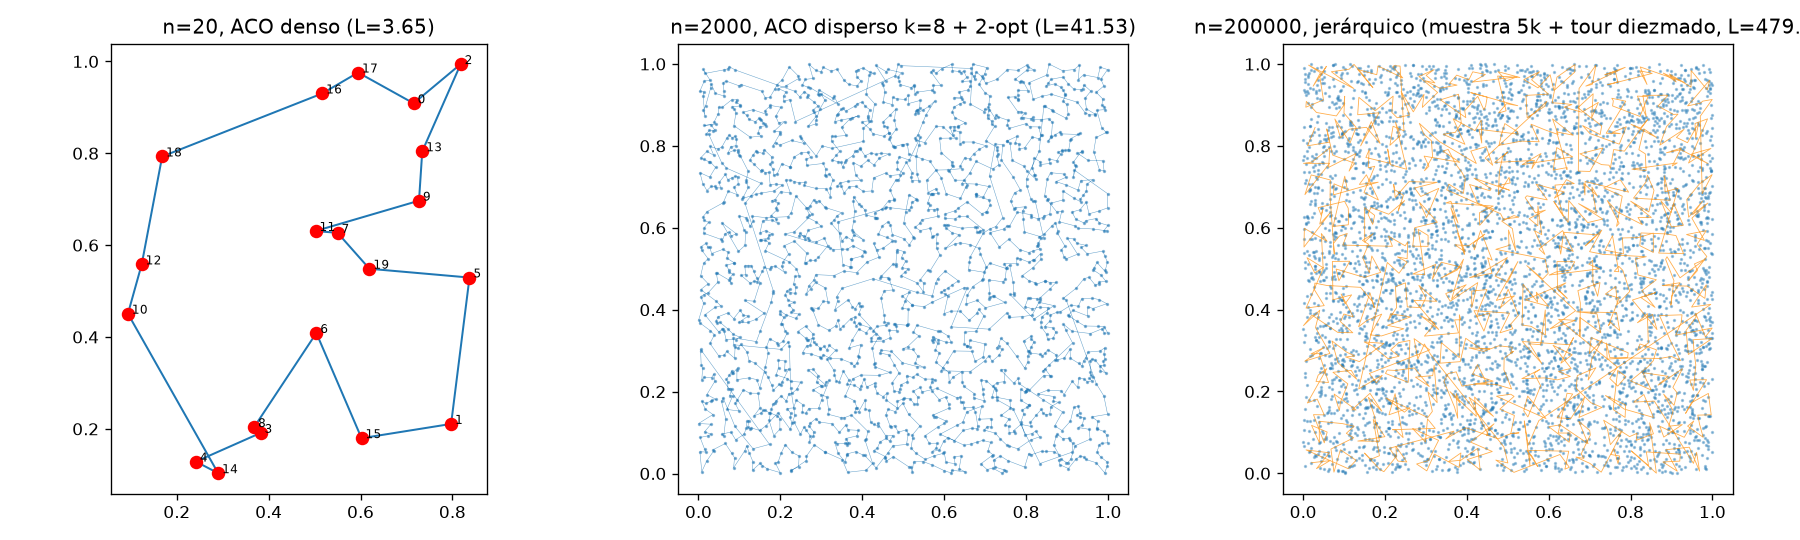
\includegraphics[width=\textwidth]{img/fig_tours.png}
\caption{Tours del ACO (recorrido \textbf{completo}, las 200.000 aristas en el panel inferior). En $N=20$ se aprecia el ciclo cerrado sin cruces innecesarios; en $N=2000$ la maraña conserva estructura local (tramos cortos entre vecinos); en $N=200.000$ se distingue la cuadrícula de $15\times15$ celdas del esquema jerárquico: cada celda se resolvió por separado y luego se cosieron por centroides. Los puntos azules tenues son las ciudades (una de cada 4) y las líneas naranjas el tour.}
\end{figure}

\begin{figure}[H]\centering
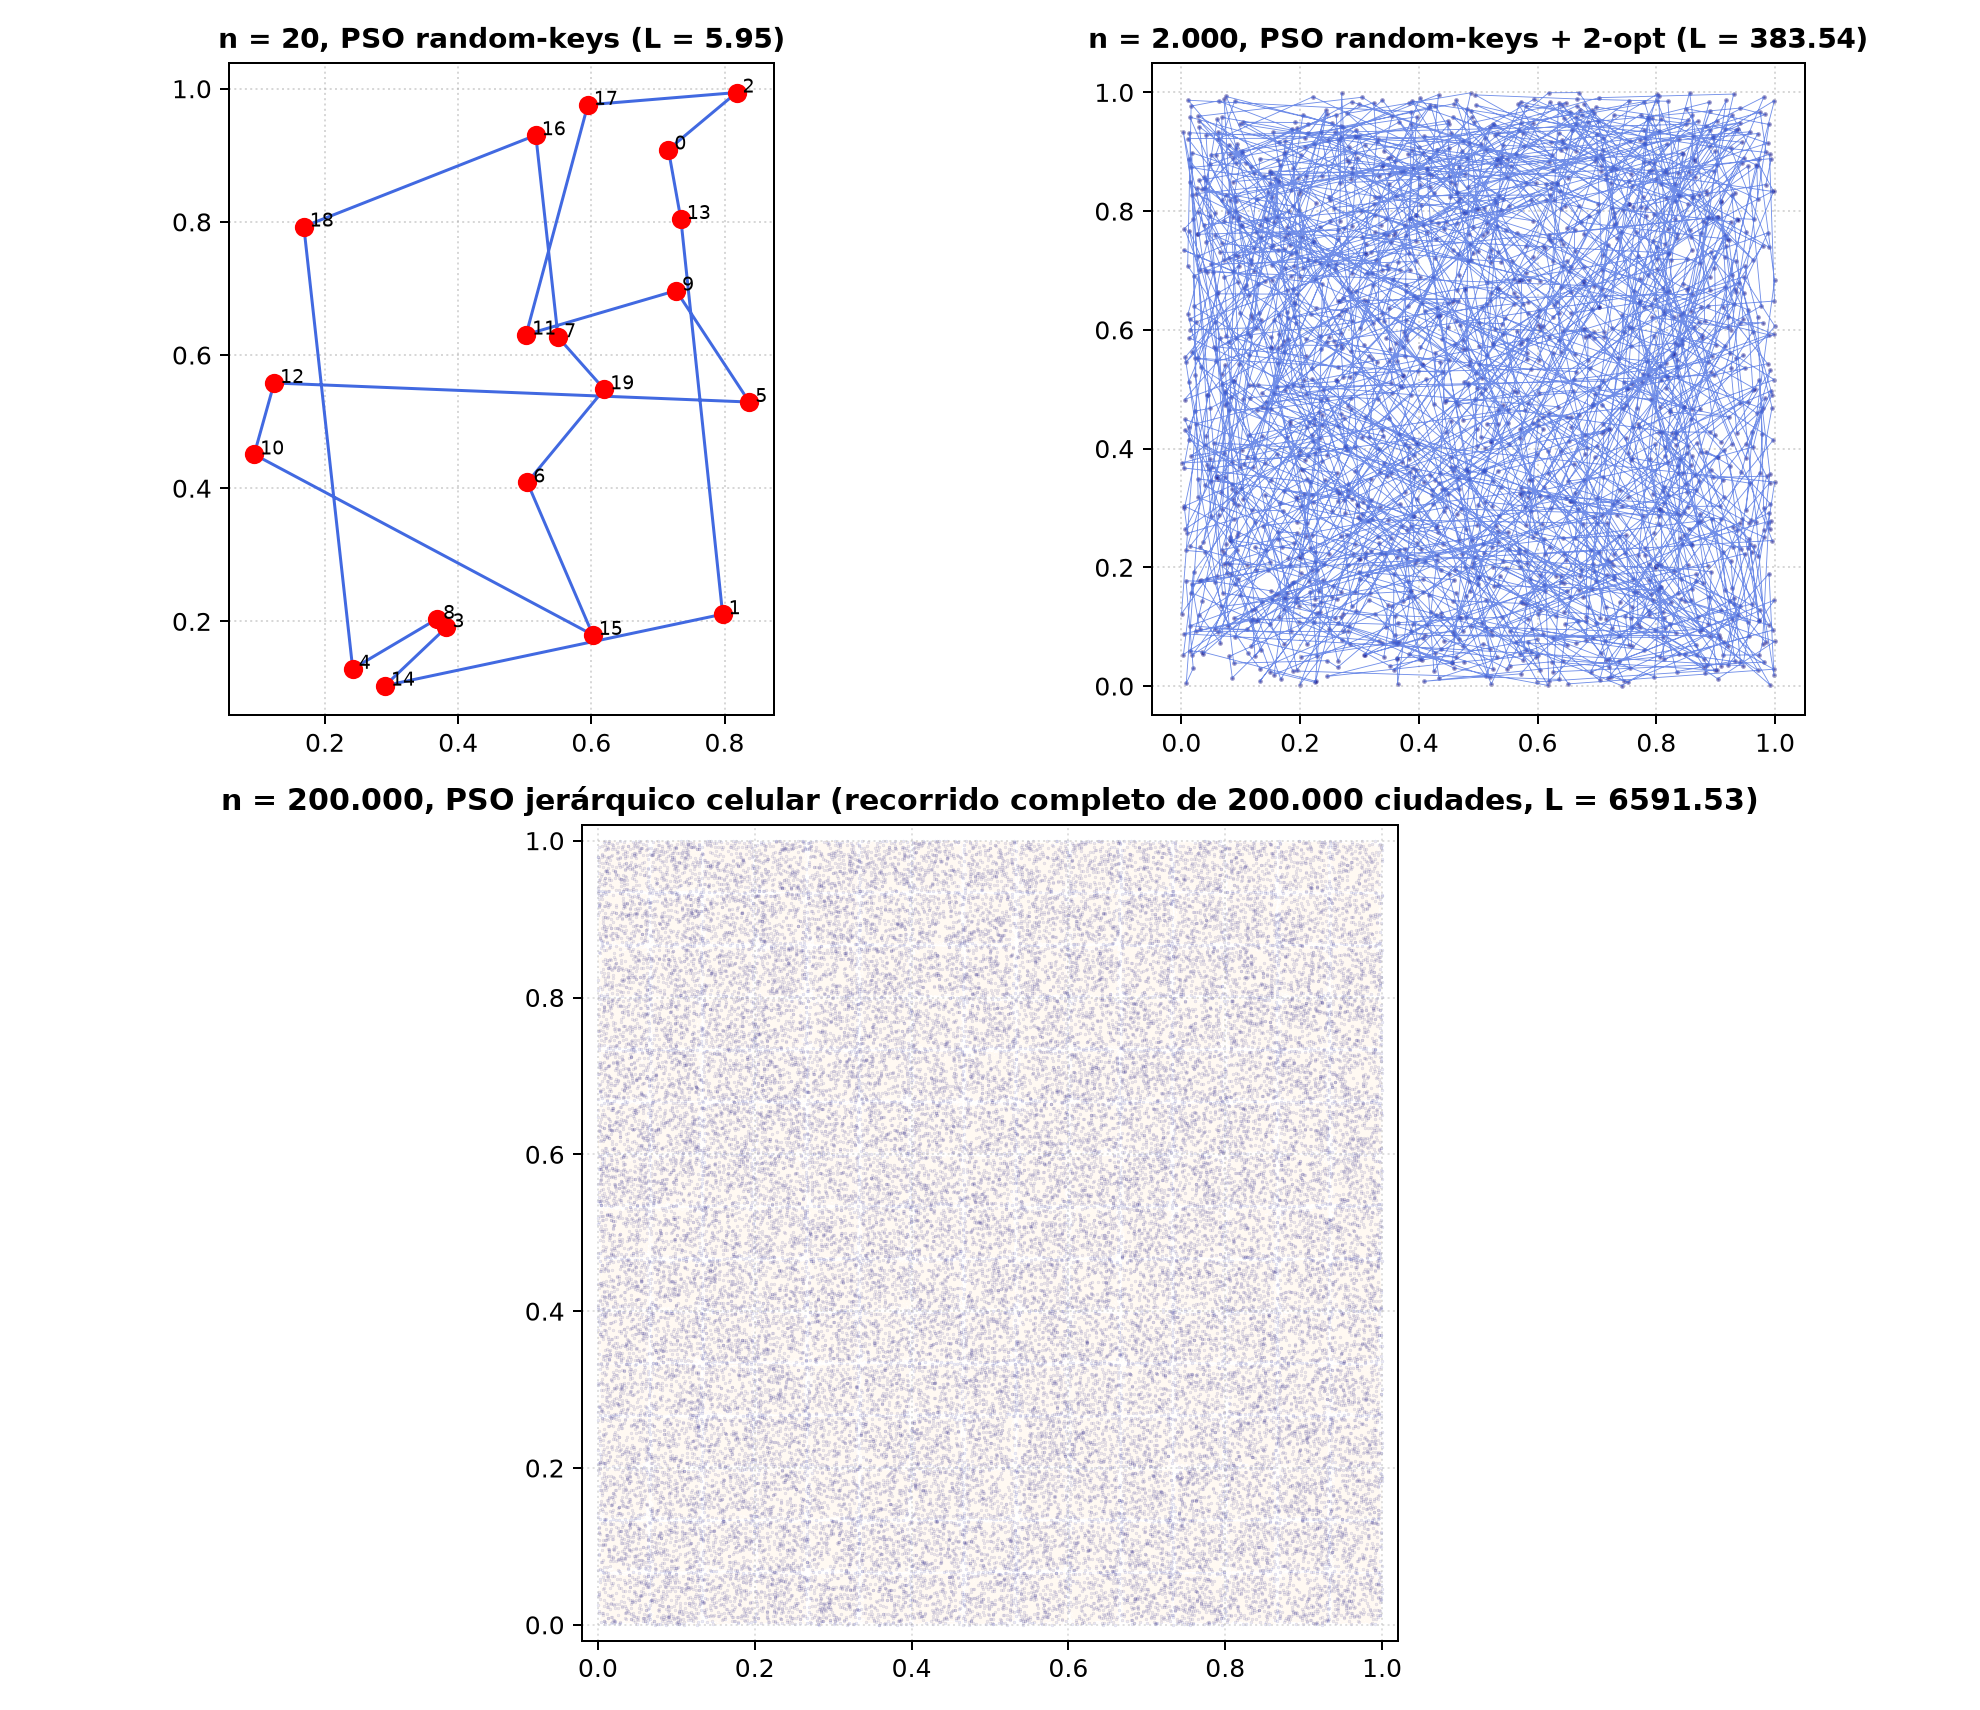
\includegraphics[width=\textwidth]{../docs/img_pso/fig_pso_tours.png}
\caption{Tours del PSO con idéntico formato. El contraste visual es el diagnóstico: en $N=2000$ predominan los segmentos que cruzan todo el cuadrado (síntoma de claves colapsadas: el orden $argsort$ deja de correlacionarse con la geografía) y en $N=200.000$ cada celda es una madeja naranja, pues el mini-enjambre por celda ($32\times40$ evaluaciones) apenas supera un tour aleatorio. Mismo andamiaje, peor motor.}
\end{figure}

\begin{figure}[H]\centering
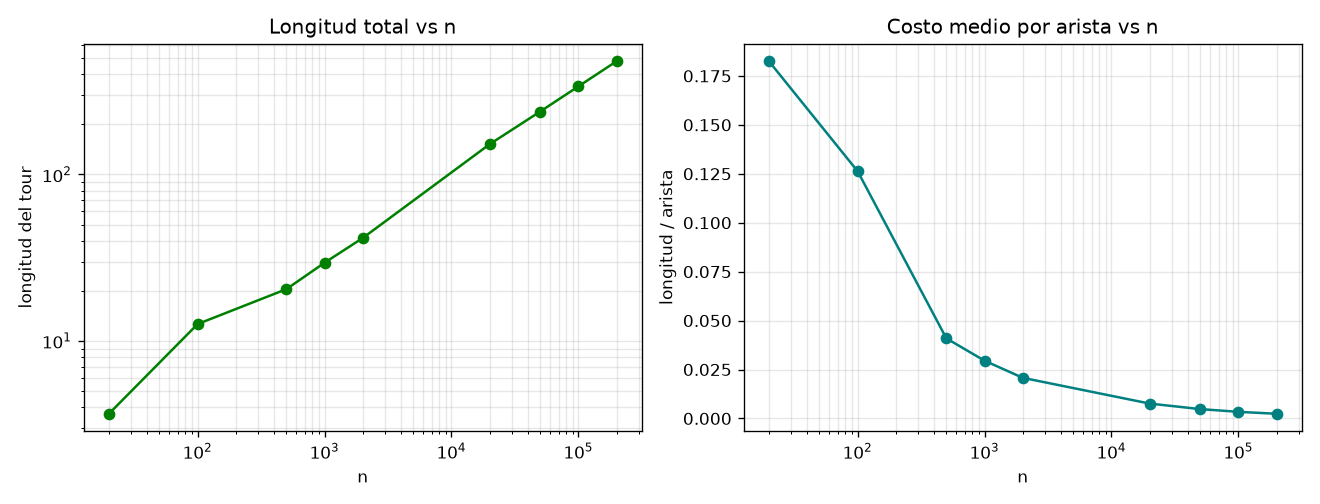
\includegraphics[width=.48\textwidth]{img/fig_calidad.png}\hfill
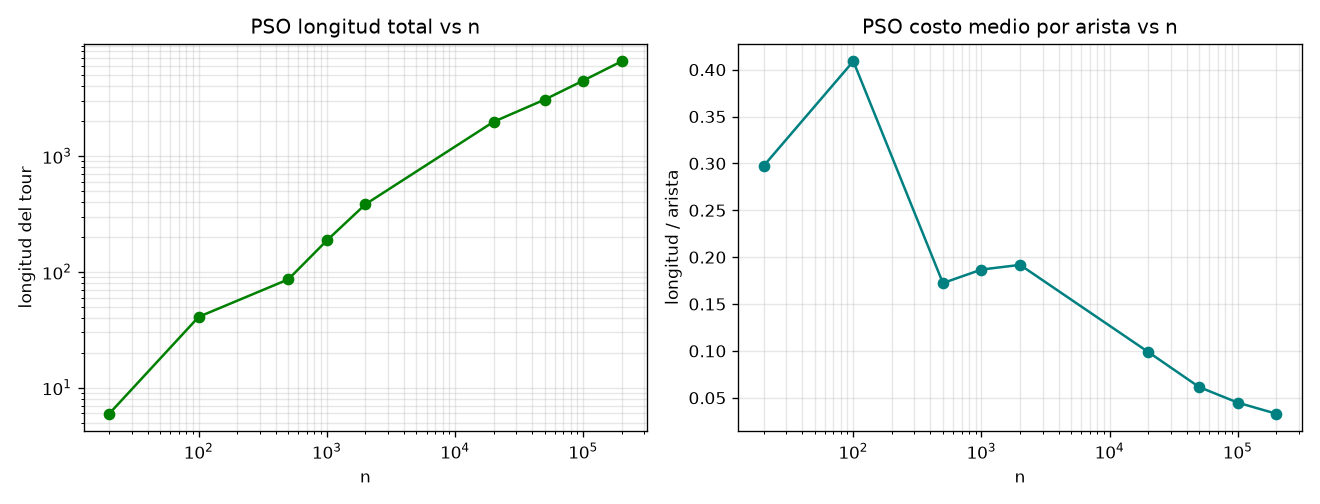
\includegraphics[width=.48\textwidth]{../docs/img_pso/fig_pso_calidad.png}
\caption{Longitud total (izq. de cada par, log-log) y costo medio por arista $L/N$ (der., semi-log). En el ACO, $L/N$ se mantiene en el orden de $10^{-3}$--$10^{-2}$ en todas las escalas: los tours son \textit{sanos} (cada arista recorre distancias locales). En el PSO, $L/N$ se degrada un orden de magnitud al crecer $N$: cada arista cruza en promedio una fracción creciente del cuadrado, la firma de un tour sin estructura. Esta gráfica es la que invalida al PSO aunque su tiempo sea menor.}
\end{figure}

\begin{figure}[H]\centering
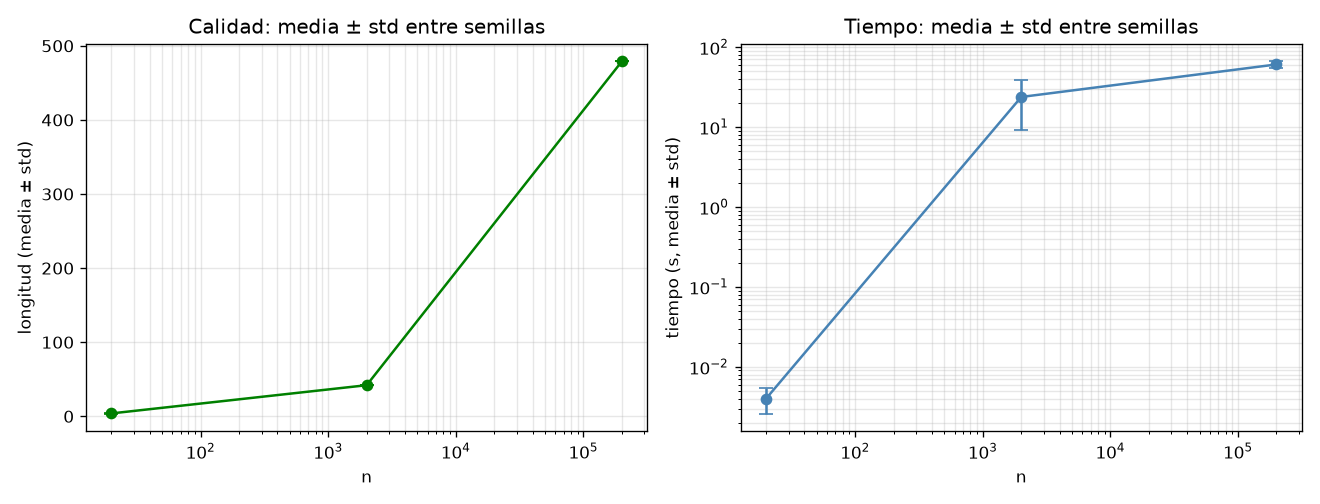
\includegraphics[width=.48\textwidth]{img/fig_semillas.png}\hfill
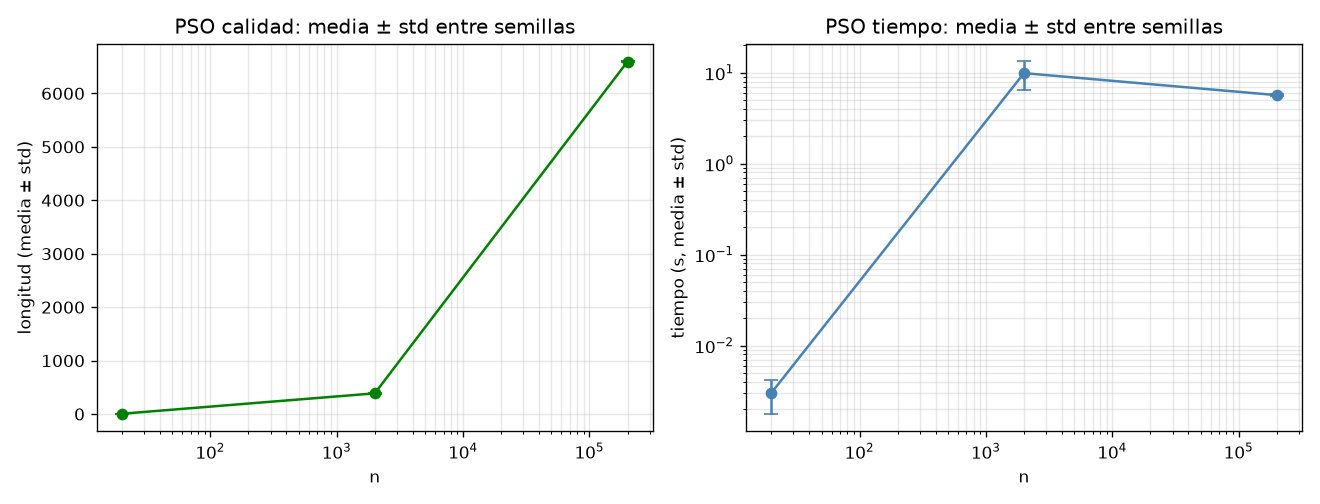
\includegraphics[width=.48\textwidth]{../docs/img_pso/fig_pso_semillas.png}
\caption{Robustez multi-semilla (§23 de ambas guías): media $\pm$ desviación de longitud y tiempo. Las barras de error del ACO son pequeñas ($\pm1\%$ en calidad), señal de un método estable; las del PSO también lo son, pero alrededor de un valor malo: ambos son estables, solo uno es bueno. La barra de tiempo del ACO en $N=2000$ es ancha (14--41\,s) porque la parada temprana $S$ dispara distinto según la semilla, ahorrando hasta 65\% de cómputo con igual calidad.}
\end{figure}

% ==============================================================================
\section{Discusión: lo que decide es el diseño, no la sigla}
% ==============================================================================
La comparación pura en $N{=}20$ (sin 2-opt en ningún algoritmo) aísla el motor metaheurístico: el ACO (3.65) supera al PSO (5.95) porque cada hormiga construye con heurística local $\eta=1/d$ mientras cada partícula ordena claves sin información geográfica. Las ablaciones lo confirman: sin feromona ($\alpha{=}0 \to 4{.}58$) ni sin heurística ($\beta{=}0 \to 6{.}56$) el ACO se degrada, y sin memoria colectiva ($c_2{=}0 \to 8{.}26$) el PSO colapsa. En general, un PSO \textbf{discreto} (operadores sobre permutaciones, arranque desde vecino más cercano y 2-opt por partícula) puede competir e incluso vencer a un ACO básico; simétricamente, el ACO aquí usado ($m{=}n$, doble feromona, elitismo) supera a un PSO continuo de arranque ciego. La moraleja es estable: la representación, el arranque y la búsqueda local aportan más que la etiqueta del algoritmo.

% ==============================================================================
\section{Conclusiones}
% ==============================================================================
\begin{enumerate}
\item Con igualdad estricta de presupuesto e instancias, el \textbf{ACO vence en calidad en las tres escalas} (exceso 24\%/0.2\%/0.1\% frente a 90\%/850\%/1294\%) a cambio de $3$--$6\times$ más tiempo de muro; en memoria empatan por debajo de $12\text{ MB}$.
\item Lo decisivo es la \textbf{representación}: construir tours con heurística local ($\eta=1/d$) aporta un buen punto de partida desde la iteración 1, mientras que ordenar claves aleatorias no induce vecindad útil y el enjambre colapsa. Para TSP discreto, colonia $>$ enjambre.
\item El ahorro de recursos es arquitectónico y compartido: sin matrices densas, feromona dispersa $O(N{\cdot}k)$ o enjambre por celdas, parada temprana por estancamiento y paralelismo por celdas independientes, $200.000$ ciudades se resuelven en $<1$ minuto con $<12\text{ MB}$ donde el enfoque ingenuo exigiría $160\text{ GB}$.
\item El PSO solo se justifica si el tiempo de muro es crítico y la calidad negociable; su valor aquí es didáctico: demuestra cuantitativamente por qué un optimizador continuo mal adaptado no compite en un problema combinatorio.
\end{enumerate}

\section*{Reproducibilidad}
\begin{verbatim}
python3 scripts/comparar_aco_pso.py   # data/comp_*.csv + docs/img_comp/*.png
\end{verbatim}
Entradas: \texttt{bin/aco}, \texttt{bin/pso} (sin modificar). Este PDF: \texttt{Informe\_Tecnico/comparativa\_aco\_pso.tex}.
\end{document}
